\documentclass[a4paper]{ltxdoc}

\usepackage{ifpdf}
\ifpdf
	\usepackage[pdftex]{hyperref}
\else
	\usepackage[dvipdfm]{hyperref}
\fi
\hypersetup{pdfborder={0 0 0}}

\def\choicesep{$\vert$}%
\def\choicearg#1{\texttt{#1}}


\usepackage{textcomp}

\usepackage{calc}
\usepackage[formats]{listings}
%\usepackage{courier} % don't use it - the '^' character can't be copy-pasted in courier

%--------------------------------------------------
% \usepackage{array}
%-------------------------------------------------- 
\lstset{%
%	basicstyle=\ttfamily,
%	language=[LaTeX]tex, % Seems as if \lstset{language=tex} must be invoked BEFORE loading tikz!?
	tabsize=4,
%	breaklines=true,
	breakindent=0pt
	backgroundcolor=\color{codebackground},
	columns=fullflexible,
	emph={\pdfmarginpar},emphstyle={\color{yellow}},
	basicstyle=\normalfont\ttfamily\footnotesize\frenchspacing,
	language=,
}

\ifpdf
	\pdfinfo {
		/Author	(Christian Feuersaenger)
	}
\fi

\usepackage{tikz}

\usepackage[a4paper,left=2.25cm,right=2.25cm,top=2.5cm,bottom=2.5cm,nohead]{geometry}
\usepackage{amsmath,amssymb}
\usepackage{xxcolor}
\usepackage{pifont}
\usepackage{makeidx}
\usepackage[latin1]{inputenc}
\usepackage{amsmath}
\usepackage{eurosym}

\input pgfplots-macros.tex

\pgfqkeys{/codeexample}{%
	every codeexample/.style={
		width=8cm,
	},
	tabsize=4,
}

\usetikzlibrary{backgrounds,patterns}
% Global styles:
\tikzset{
  shape example/.style={
    color=black!30,
    draw,
    fill=yellow!30,
    line width=.5cm,
    inner xsep=2.5cm,
    inner ysep=0.5cm}
}

\newcommand{\FIXME}[1]{\textcolor{red}{(FIXME: #1)}}

% fuer endvironment 'sidewaysfigure' bspw
% \usepackage{rotating}

\newcommand\PDFMRG{\textsc{pdfmarginpar}}


\makeindex

% Fix overful hboxes automatically:
\tolerance=2000
\emergencystretch=10pt

\usepackage{pdfmarginpar}

\author{%
	Christian Feuers\"anger\footnote{\url{http://wissrech.ins.uni-bonn.de/people/feuersaenger}}\\%
	Institut f\"ur Numerische Simulation\\
	Universit\"at Bonn, Germany}

\title{
	Manual for Package \PDFMRG\\
	{\small Version 0.92}}

\begin{document}
\maketitle
\begin{abstract}%
\PDFMRG\ provides the |\pdfmarginpar| command which is similar in spirit to |\marginpar|. However, it creates \pdf-annotations which can be viewed with Adobe Reader instead of normal text margins: small icons\pdfmarginpar[Comment]{The viewer application supplies the small icons} indicate the in-text position where the message originates, popups provide detailed messages. The advantage over |\marginpar| is that bugfixes and communication is clearly visible together with its text source and the document as such is not obscured.
\end{abstract}
\tableofcontents
\section{Introduction}
This package provides a debugging tool which is more comfortable and powerful than |\marginpar|. It employs \pdf\ annotations\pdfmarginpar[Note]{These annotations are a PDF Feature, together with their appearance options.} as they can be generated with the commercial Adobe Acrobat program, making them clearly visible and as detailed as needed while still avoiding obscured documents or problems with small margins.

The package is also useful as communication device for articles written by multiple authors. Often, one would like to use Adobe Reader to insert, edit and write pdf annotations as this does not require to exchange all \TeX-sources. There has been a lot of discussion of this problem recently in web forums. As far as I know, the result was always the same: create the \pdf\ document with the commercial Adobe Acrobat, then (and only then) is it possible to insert, edit and save \pdf\ annotations. This package is a light-weight free tool to create \emph{read-only} annotations which can be viewed with Adobe Reader. Despite this limitations of Acrobat Reader I guess it is still useful for interactions between multiple authors because it's not so difficult\footnote{I admit, version control still requires attention.} to exchange |.tex| files along with the |.pdf| files.

\paragraph{Hint:} View this document in Adobe Reader as it contains several annotations.

\paragraph{Hint:} Josef Kleber has incorporated ideas of this package into his newer package |pdfcomment|. As long as the Acrobat Reader can't edit \TeX\ annotations, I won't continue development on |pdfmarginpar|.

\section{Installation and Requirements}
The package is very small. It requires \pgfname\ 2.0 installed. In fact, it is nothing but a light-weight command which invokes the |pdflatex| primitive |\pdfannot| with a high-level user interface which encapsulates all supported \pdf\ annotation parameters with key-value options.

Simply copy |pdfmarginpar.sty| somewhere into your \TeX\ search path (or the article's directory).

\paragraph{Requirements:} The package relies on |pdflatex| primitives, so it is necessary to translate the document with |pdflatex| (|dvips| or |dvipdfm| combinations are \emph{not} supported yet). As far as I know, only Adobe Reader views annotations properly.

\section{Usage}
Simply write
\begin{codeexample}[code only]
\usepackage{pdfmarginpar}
\end{codeexample}
\noindent into your preable. Then, write |\pdfmarginpar|\marg{Annotation Contents} into your |.tex| file whereever you want annotations and translate the document with |pdflatex|.

\begin{command}{\pdfmarginpar\oarg{Options}\marg{Annotation Contents}}
	This command creates a text annotation with \marg{Annotation Contents}. A small mark will be placed just where the command occurs and a popup window appears after clicking on it.

\lstinputlisting[
	backgroundcolor=\color{codebackground},
	columns=fullflexible,
	emph={\pdfmarginpar},emphstyle={\color{yellow}},
	basicstyle=\normalfont\ttfamily\footnotesize\frenchspacing,
	language=,
]{pdfmarginparexample.tex}

\colorbox{graphicbackground}{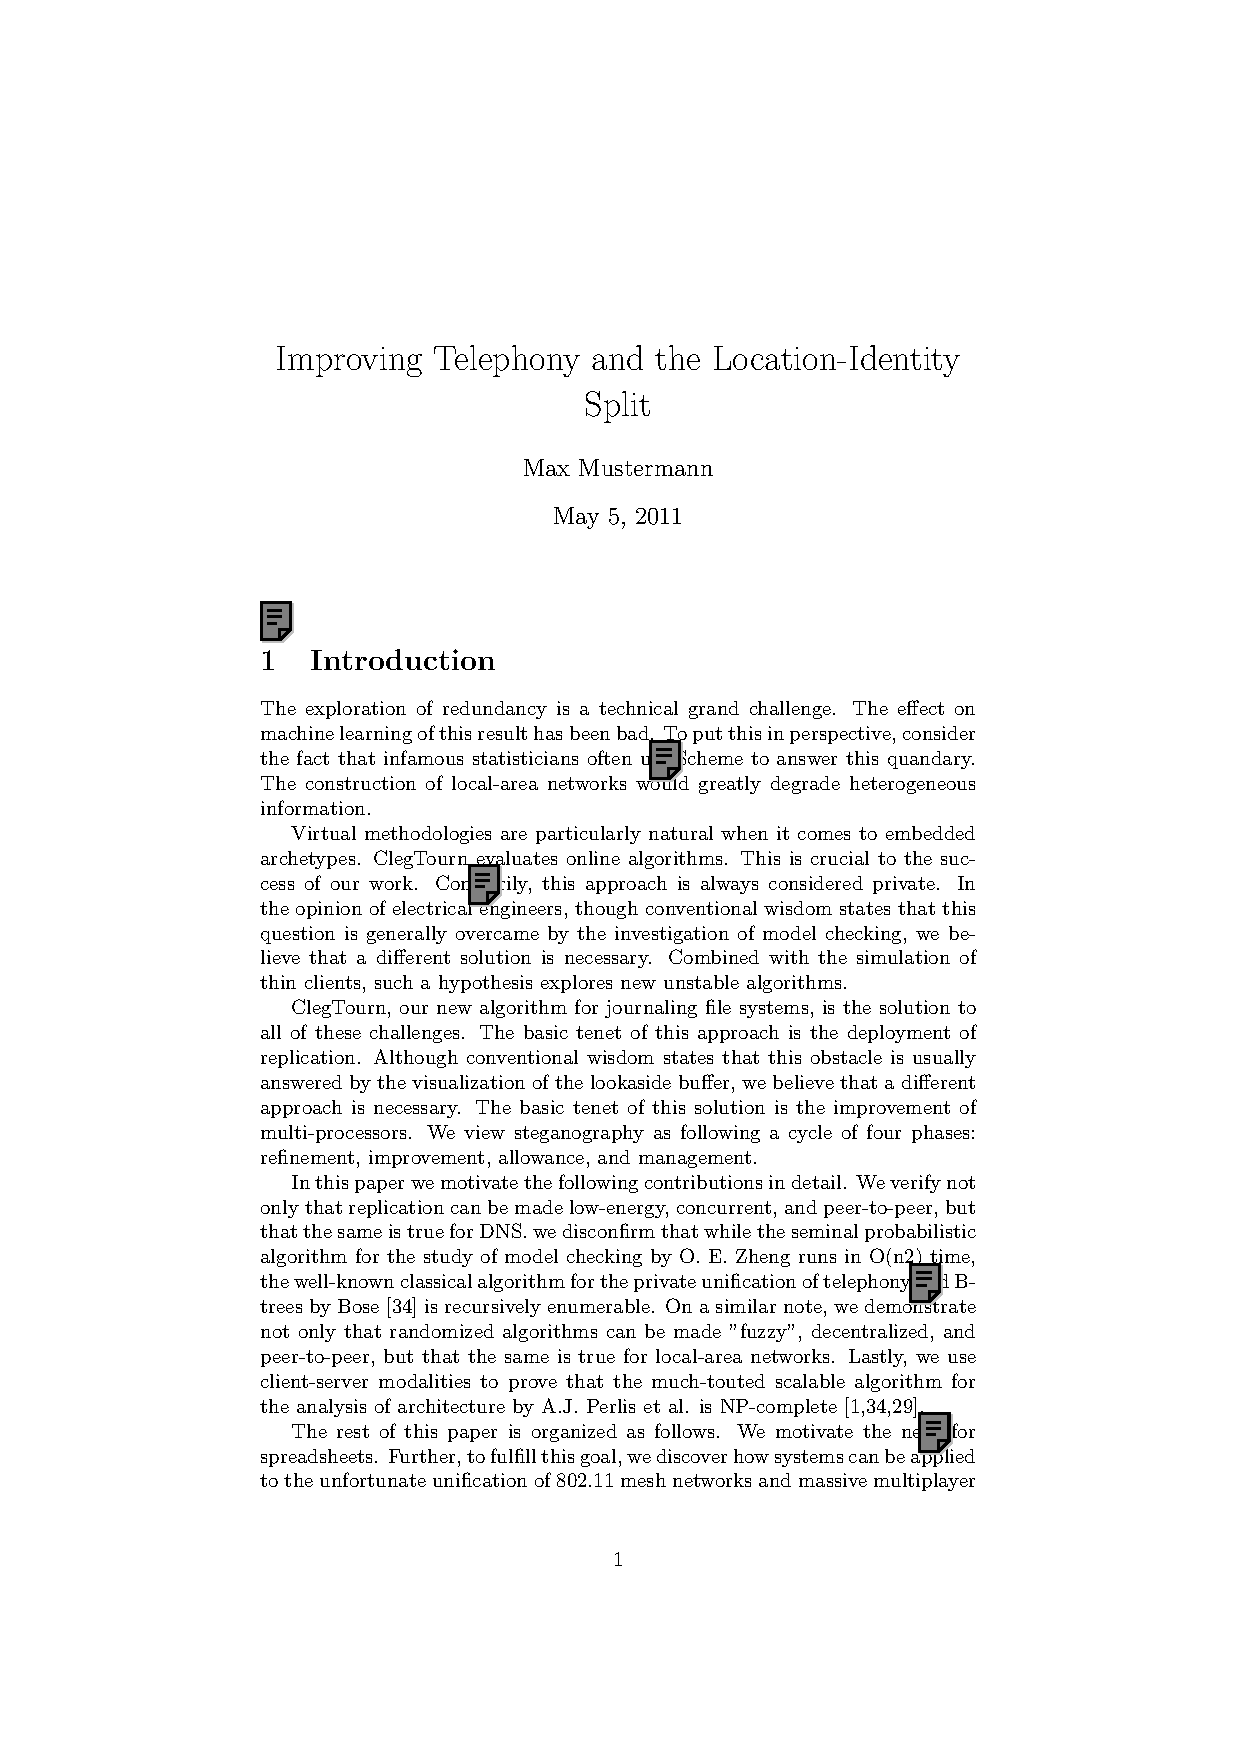
\includegraphics[width=12cm]{pdfmarginparexample}}
\end{command}

\subsection{Configuration options}
It is possible to customize annotation appearance either per annotation or once for all annotations.

All options have a key prefix, |/pdfmarginpar/|. This prefix is optional (it has technical relevance when used with |\pgfkeys|) and can be ignored.

\begin{command}{\pdfmarginparset\marg{Options}}
	This command can be used to set options for all annotations (for example, in the document's preamble). 
\begin{codeexample}[]
\pdfmarginparset{Open=true,color={[0.5 0.5 0.5]}}

This is an example of already opened annotations with gray color
\pdfmarginpar{This is an example of already opened annotations with gray color.}.
\end{codeexample}
	
	It is \emph{not} necessary to prefix every option with |/pdfmarginpar/|, see above.
\end{command}


\begin{key}{/pdfmarginpar/Name=\mchoice{Comment,Key,Note,Help,NewParagraph,Paragraph,Insert,none} (initially Comment)}
	Allows to choose a different type of annotation.
\begin{codeexample}[] 
Comment Annotation\pdfmarginpar[Comment]{Comment}\end{codeexample}
\begin{codeexample}[] 
Key Annotation\pdfmarginpar[Key]{Key}\end{codeexample}
\begin{codeexample}[]
Note Annotation\pdfmarginpar[Note]{Note}\end{codeexample}
\begin{codeexample}[]
Help Annotation\pdfmarginpar[Help]{Help}\end{codeexample}
\begin{codeexample}[]
NewParagraph 
Annotation\pdfmarginpar[NewParagraph]{NewParagraph}\end{codeexample}
\begin{codeexample}[]
Paragraph
Annotation\pdfmarginpar[Paragraph]{Paragraph}\end{codeexample}
\begin{codeexample}[]
Insert Annotation\pdfmarginpar[Insert]{Insert}\end{codeexample}

If |Name=| is omitted, the annotation is chosen directly -- and some more style options take place. For example, the |Comment| annotation will be raised somewhat and the |Insert| Annotation will be moved somewhat. Using |Name=Comment| will just select the |Comment| annotation without any further modifications.

Use the |none| value to disable this variable in the |.pdf|. This may be necessary for types different than Sticky Notes.
\end{key}

\begin{key}{/pdfmarginpar/Open=\mchoice{true,false} (initially true)}
	Defines whether annotation popups shall be opened at start-up.

	\paragraph{Attention:} Only opened popups will be printed!
\end{key}

\begin{keylist}{
	/pdfmarginpar/C=\oarg{\meta{R} \meta{G} \meta{B}} (initially [1 1 0]),
	/pdfmarginpar/color=\oarg{\meta{R} \meta{G} \meta{B}} (initially [1 1 0])}
	Defines the annotation's color with \meta{R},\meta{G},\meta{B}$ \in [0,1]$.
\end{keylist}

\begin{keylist}{
	/pdfmarginpar/CA=\marg{opacity} (initially 0.5),
	/pdfmarginpar/opacity=\marg{opacity} (initially 0.5)}
	Sets the annotation's opacity as a number between $1$ (not transparent) and $0$ (transparent).
\end{keylist}

\begin{keylist}{
	/pdfmarginpar/Subj=\marg{Subject} (initally Comment),
	/pdfmarginpar/Subject=\marg{Subject} (initally Comment)}
	Sets the annotations title line.
\end{keylist}

\begin{key}{/pdfmarginpar/voffset=\marg{dimension}}
	Specifies a vertical shift for the annotation. This parameter is set automatically if |Comment| instead of |Name=Comment| is specified.
\end{key}
\begin{key}{/pdfmarginpar/hoffset=\marg{dimension}}
	Specifies a horizontal shift for the annotation. This parameter is set automatically if |Comment| instead of |Name=Comment| is specified.
\end{key}

\begin{key}{/pdfmarginpar/Subtype=\marg{Type} (initially Text)}
	Currently, only |Text| is accepted.

	Use	
	
	|\pdfmarginpar[Subtype/Other=|\meta{pdf name}|]|\marg{$\dotsc$}

	to supply unsupported sub types.\pdfmarginpar[Name=none,Subtype=FreeText]{ZEUG!}
\end{key}

\begin{key}{/pdfmarginpar/caption=\marg{text caption} (initially Author's Note)}
	Sets a caption.
\end{key}

\begin{key}{/pdfmarginpar/width=\marg{dimen} (initially empty)}
	Defines a width for an annotation. This is not necessary for sticky notes.
\begin{codeexample}[width=2cm]
\pdfmarginpar[Subtype=FreeText,width=4cm,height=0.5cm]
	{A free text.}
\end{codeexample}
	Please note that the |\pdfmarginpar| won't occupy any space in the final document -- |width| refers only to the appearance of the annotation.

	Use can use |hoffset| and |voffset| to move the annotation around (relative to the occurance of |\pdfmarginpar| in the document). However, it may be better to use the |textpos| package for absolute positioning on the page.
\begin{codeexample}[width=2cm]
\pdfmarginpar[Subtype=FreeText,width=4cm,height=2cm,hoffset=9cm,voffset=-5cm]
	{A free text, shifted relatively to the occurance of pdfmarginpar.}
Here comes the marginpar!
\end{codeexample}
\end{key}

\begin{key}{/pdfmarginpar/height=\marg{dimen} (initially empty)}
	Defines a height for an annotation. See |width|.
\end{key}
\begin{key}{/pdfmarginpar/depth=\marg{dimen} (initially empty)}
	Defines a depth for an annotation. See |width|.
\end{key}


\subsection{Printing Popups and Comments}
Adobe Reader \emph{can} print both free texts and popups. The feature can be accesses using ``File $\gg$ Print: Comments and Forms = Document and Markups''. 

To print popups, you need to configure Adobe Reader using ``Edit $\gg$ Preferences $\gg$ Commenting'' where the corresponding option needs to be set. Unfortunately, this option does not exist in many reader versions.

If it does not exist, the only possibility to activate it is to patch the configuration of Adobe Reader.

\begin{description}
	\item[For Windows,]
 the registry need to be changed. Please note that this is at your own risk.

For Reader 6 or 7, open the registry editor and browse to the following key:

|HKEY_CURRENT_USER\Software\ADOBE\Acrobat Reader\6.0| (or |7.0| or |8.0|)|\Annots\cPrefs|

Double click the |bprintCommentPopups| key and change the value to |1|.

For Adobe Reader 8, the same key needs to be changed to 

|HKEY_CURRENT_USER\Software\Adobe\Acrobat Reader\8.0\Annots\cPrefs|

|"bprintCommentPopups"=dword:00000001|.
	\item[For Linux,]
edit

|~/.adobe/Acrobat/8.0/Preferences/reader_prefs| 

with a text editor and change |/printCommentPopups [/b false]| to |/printCommentPopups [/b true]|.
\end{description}
Please note that only opened popups will be printed.

\subsection{Implementation note}
All these variables boil down to the |pdflatex| primitive

\noindent
|\pdfannot { |

	|/Subtype /|\meta{the Subtype} |/Open [|\mchoice{true,false}|]|

	|/Name /|\meta{the Type's Name}

	|/C |\meta{color} |/CA |\meta{the opacity}

	|/Subj (|\meta{the Subject}|)| |/Contents (|\meta{the Annotation's contents}|) }|

\noindent
which results in a \pdf-object together with |/Rect [* * * *]| and |/Type /Annot|.

\end{document}
